\documentclass[a4paper, 12pt]{article}
\usepackage{geometry}
\geometry{margin=2cm}
\usepackage[indonesian]{babel}
\usepackage{setspace}
\onehalfspacing{}
\usepackage{hyperref}
\usepackage{float}
\hypersetup{
    colorlinks,
    citecolor=black,
    filecolor=black,
    linkcolor=blue,
    urlcolor=blue
}

\usepackage{graphicx}
\graphicspath{./images/}
\title{\textbf{Tugas Perorangan}\linebreak
\textbf{Rekayasa Jaringan CCTV di Komplek Perumahan}\linebreak}
\date{}

\usepackage{subfiles}
% \usepackage{indentfirst}
\setlength{\parindent}{20pt}
\begin{document}
\subfile{./subfiles/cover.tex}

% \tableofcontents
% \thispagestyle{empty}
% \pagebreak
\clearpage
\setcounter{page}{1}
\section{Perumusan Masalah}
Diberikan sebuah kejadian pada komplek XYZ yang akan membuat sistem Keamanan Lingkungan menggunakan CCTV dengan ketentuan:
\begin{enumerate}
  \item Server atau Tempat untuk melakukan monitoring CCTV bisa disimpan di pos satpam dan GSG\dots
  \item jalan yang pendek hanya dipasang 1 unit CCTV pada salah satu ujung jalan tsb\dots
  \item jalan yang panjang dipasang 2 unit CCTV pada kedua ujung jalan tsb\dots
  \item jalan yang panjang yaitu:
    \begin{itemize}
      \item Dari Pos Satpam ke ujung taman\dots
      \item Antara Blok A dan C\dots
      \item Antara Blok C depan dan C belakang\dots
      \item Blok E\dots
      \end{itemize}
  \item Di dalam masjid dipasang 1 unit CCTV\dots
  \item buatlah jaringan Sistem Keamanan Lingkungan Komplek XYZ 
\end{enumerate}
dengan gambar yang disediakan sebagai berikut:
\begin{figure}[ht]
  \begin{center}
    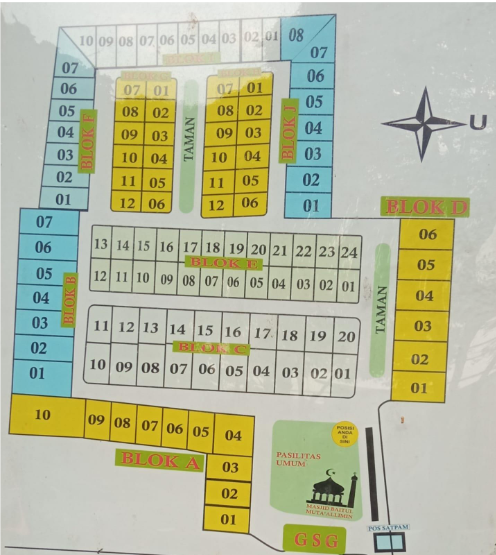
\includegraphics[width=0.5\textwidth]{images/peta.png}
  \end{center}
  \caption{Peta}\label{fig:peta}
\end{figure}
\pagebreak
\section{Pemetaan}
Berdasarkan informasi yang ada maka dapat dipetakan sebagai berikut:
\begin{figure}[ht]
  \begin{center}
    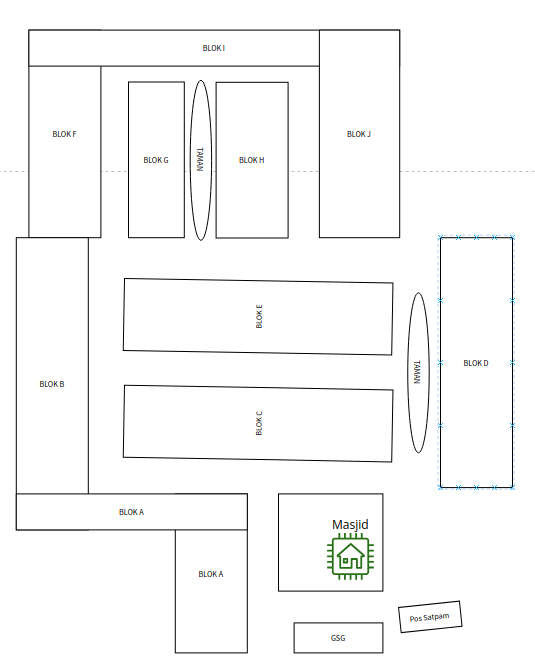
\includegraphics[width=0.5\textwidth]{images/layout.png}
  \end{center}
  \caption{textbf{Gambar 2}. denah simpel}\label{fig:denah}
\end{figure}
dengan gambar \ref{fig:denah} diatas dapat diperhitungkan bagaimana lokasi penempatan dari CCTV yang akan dipasang di perumahan XYZ ini, untuk servernya dapat disimpan di pos satpam agar memudahkan dalam mengakses sistem keamanan ini.
\pagebreak
\begin{figure}[hb!]
  \begin{center}
    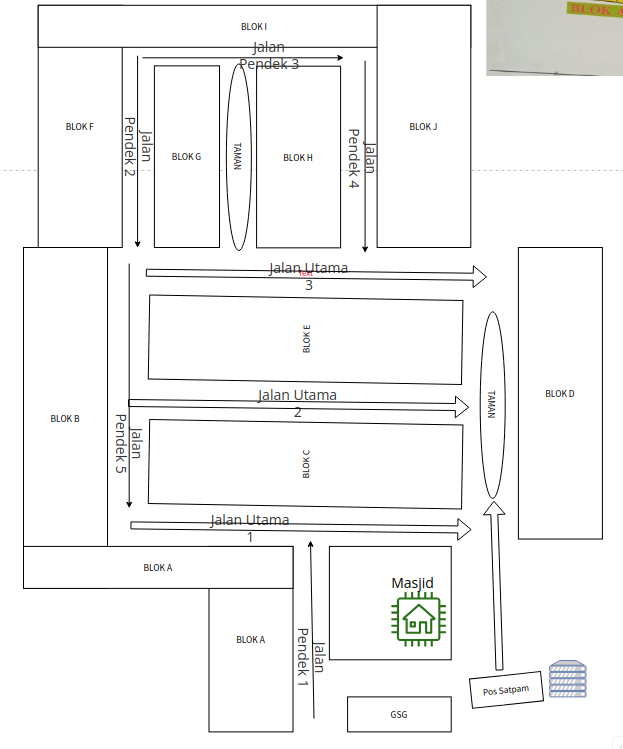
\includegraphics[width=0.5\textwidth]{images/cctv.png}
  \end{center}
  \caption{Denah perumahan}\label{fig:cctv}
\end{figure}
berdasarkan gambar \ref{fig:cctv} dapat digambarkan secara mudah bagaimana pembagian jalan yang ada di perumahan XYZ ini untuk nantinya penempatan CCTV, dengan penjelasan sebagai berikut:
\begin{enumerate}
  \item jalan Panjang ada 3 yakni Jalan utama 1,2,3 dan area dari satpam menuju taman berdasarkan informasi diatas sehingga dibutuhkan 2 CCTV di setiap ujung jalannya\dots
  \item jalan Pendek ada 5 yakni jalan pendek 1,2,3,4,5 yang menjadi jalan yang memiliki ukuran yang pendek sehingga hanya diperlukan satu CCTV saja\dots
  \item Masjid diharuskan memiliki CCTV untuk alasan keamanan dari fasilitas umum\dots
\end{enumerate}
berdasarkan informasi diatas maka dapat digambarkan sebagai berikut:
\begin{figure}[H]
  \begin{center}
    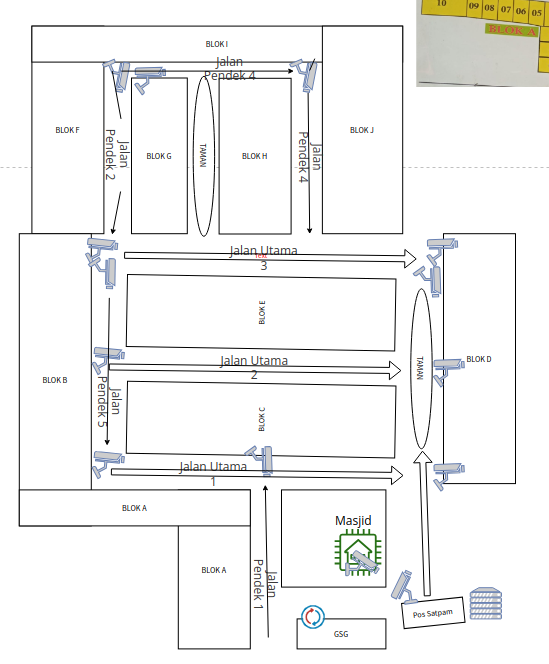
\includegraphics[width=0.5\textwidth]{images/jalan.png}
  \end{center}
  \caption{Lokasi CCTV}\label{fig:jalan}
\end{figure}
berdasarkan gambar \ref{fig:jalan} dapat dijelaskan bagaimana CCTV yang akan dipasang di perumahan XYZ ini yang kemudian dapat dijabarkan bagaimana jaringan sistem ini dapat berjalan seperti;
\begin{figure}[H]
  \begin{center}
    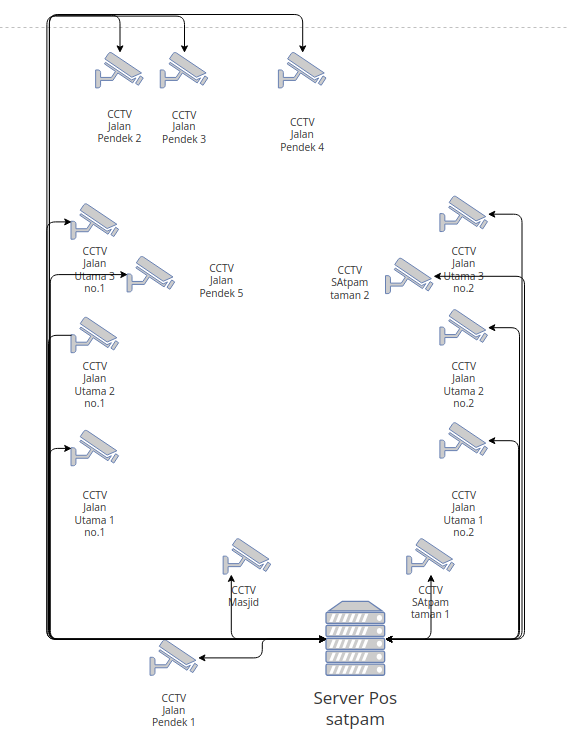
\includegraphics[width=0.5\textwidth]{images/sistem.png}
  \end{center}
  \caption{jaringan}\label{fig:jaringan}
\end{figure}
dengan penjelasan sebagai berikut:
\begin{enumerate}
  \item Server disimpan di pos satpam untuk kemudahan mengaksesnya\dots
  \item untuk koneksinya dibagi menjadi dua sisi yakni sisi kanan dan kiri untuk memudahkan dalam memeliharanya dan memudahkan untuk membuat jalurnya\dots
  \item bagian kiri ada beberapa CCTV yakni:
    \begin{itemize}
      \item CCTV masjid
      \item CCTV jalan pendek 1
      \item CCTV jalan pendek 2
      \item CCTV jalan pendek 3
      \item CCTV jalan pendek 4
      \item CCTV jalan pendek 5
      \item CCTV jalan utama 1 no 1
      \item CCTV jalan utama 2 no 1
      \item CCTV jalan utama 3 no 1
    \end{itemize}
  \item untuk bagian kanan ada beberapa CCTV yakni:
    \begin{itemize}
      \item CCTV satpam taman 1
      \item CCTV satpam taman 2
      \item CCTV jalan utama 1 no 2
      \item CCTV jalan utama 2 no 2
      \item CCTV jalan utama 3 no 2
    \end{itemize}
\end{enumerate}
\end{document}

